\section{Methodology}
To generate CPU stress, we used sysbench \cite{sysbench}, which is a powerful cross-architecture tool
that can be used for Linux performance benchmarks. As a CPU stress-testing tool, it deterministically 
checks all prime numbers up to 10,000 (default value) by dividing each candidate number by all integers 
from 2 up to its square root \cite{gentoo_sysbench}. The number of worker threads 
as well as the aggregated workload of the created threads can be specified as arguments. 
The total execution runtime is then used as a comparison metric 
between the different experiments. For comparison purposes, we also developed our CPU stressing 
tool called \textit{cpu\_burn} written in the C language. The program takes two arguments, the first 
being the number of operations that each created thread will perform, and the second representing 
the number of worker threads. It outputs the total wall-clock runtime that was needed for the 
execution of this job. 
We compiled the program using GCC with optimization level -O0, to ensure no compiler optimizations
altered the program's behavior. Each thread executes the function defined under \texttt{perform\_work()}. 
As stated previously, The argument \texttt{work->operations} is specified by the user.

\begin{figure}[H]
\begin{lstlisting}[caption={Workload of the \textit{cpu\_burn} tool}]
void* perform_work(void* arg) {
    ThreadWork* work = (ThreadWork*)arg;
    double x = 0.0;
    for (long long i = 0; i < work->operations; ++i) {
        x += i * 0.000001;
    }
    work->result = x;
    return NULL;
}
\end{lstlisting}
\end{figure}
\noindent
This section investigates CPU contention on general-purpose instances from 5th and 6th EC2 generations, 
with different CPU architectures. We analyzed the potential degradation on hosts that support 
\acl{SMT}: namely m5, m6i and m6a hosts. We then considered the single-threaded AWS Graviton 2 
processor used by the m6g dedicated host. Key Performance Indicators are described 
in Table \ref{tab:dedicated-hosts}. We notice that the first three dedicated hosts have a number of vCPUs 
twice the number of the physical cores, as these hosts support \ac{SMT} with 
two threads per physical core. The m6g instance has the best price per vCPU ratio, although each 
vCPU is mapped to a physical and not to a logical core.

\renewcommand{\arraystretch}{1.5} % Adjust this value as needed
\begin{table}[h]
\centering
\begin{tabular}{|l|p{2cm}|p{2cm}|p{2cm}|p{2cm}|}
\hline
KPI & m5 & m6i & m6a & m6g \\
\hline
Processor \cite{cloudspecs} & Intel Xeon Platinum 8175/ Intel Xeon Platinum 8280	 & Intel Xeon 8375C & AMD EPYC 7R13 Processor & AWS Graviton2 \\
\hline
Hypervisor \cite{awsEC2GP2025} & Nitro v2 & Nitro v4 & Nitro v4 & Nitro v2 \\
\hline
vCPUs \cite{pricing} & 96 & 128 & 192 & 64 \\
\hline
Physical CPUs \cite{pricing} & 48 & 64 & 96 & 64 \\
\hline
Clock speed (GHz) \cite{vantage} & 3.1 & 3.5 & 3.6 & 2.5\\
\hline
Hypervisor \cite{hypervisorSpec} & Nitro & Nitro & Nitro & Nitro \\
\hline
price/hour \cite{pricing} & \$5.069 & \$6.758 & \$9.124 & \$2.71 \\
\hline
price/vCPU/hr & \$0.053 & \$0.053 & \$0.048 & \$0.042 \\
\hline
\end{tabular}
\caption{KPIs for AWS Dedicated Host families m5, m6i, m6a, and m6g.}
\label{tab:dedicated-hosts}
\end{table}
\noindent
The experiment is structured as follows: A node, referred to as test node 
is first deployed on the dedicated host. Next, neighbors that fully utilize their vCPUs are 
incrementally added. We analyze the effect of adding busy neighbors on the runtime of running 
cpu benchmarks on the test node.
Figure \ref{fig:cpu_exp} provides a visualization of the experiment. 
\begin{figure}[H]
  \centering
  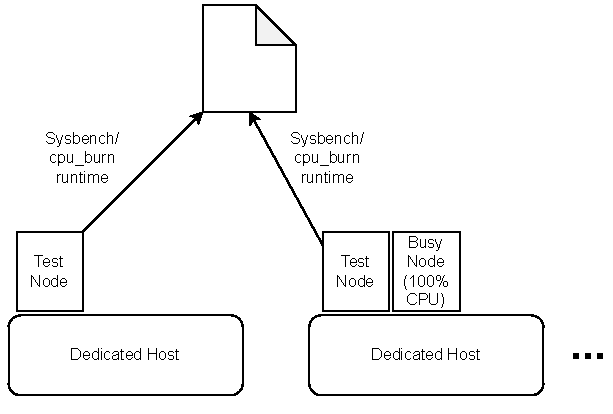
\includegraphics[width=11cm, height=7cm]{figures/cpu_exp}
  \caption{CPU contention experiment}
  \label{fig:cpu_exp}
\end{figure}
\noindent
For comparison, the experiment was repeated but with idle neighbors instead of busy. To identify the cause of the 
observed degradation, we also natively ran the benchmarking tools on the metal 
instance of each family. Metal instances run directly on the physical host without the need 
for the hypervisor. They provide the user with access to all the physical 
CPUs. The behavior of the metal instance will not be analyzed in depth, 
as it is out of the scope of the thesis. It is included solely to support a better understanding of 
CPU contention.

